\chapter{Diseño e implementación} % Main chapter title

\label{Chapter3}

En este capítulo se describe la arquitectura global del prototipo, se detalla cada módulo hardware y software que lo compone, y se documentan las decisiones de implementación, los criterios de diseño y las pruebas preliminares realizadas. Se explican los flujos de datos entre el dispositivo de campo, el broker MQTT, el backend (API REST), la interfaz web, se resumen las consideraciones para el despliegue y el monitoreo post-implantación.


\section{Arquitectura del sistema}

La arquitectura propuesta separa de forma explícita el dispositivo de campo (contador + ESP32-C3 + SIM800L), el transporte de mensajes (broker MQTT) y los servicios de aplicación (API REST, persistencia y frontend). Esta separación facilita la interoperabilidad y permite desplegar la solución de forma local, remota o híbrida según las políticas institucionales


\subsection{Flujo de datos} 

\begin{itemize}

  \item Detección: el contador detecta un paso y envía una trama por RS-232 al ESP32-C3.

  \item Preprocesado en nodo: el firmware valida la trama, añade sello temporal y metadatos, y encola el evento en memoria (FIFO).

  \item Transmisión: cuando la conexión GPRS está disponible, el nodo publica el evento en el tópico MQTT \texttt{devices/{id}/events}.
  
  \item Ingesta y persistencia: el broker Mosquitto entrega el mensaje al suscriptor backend, el servicio valida el payload y persiste el registro en la base de datos MySQL.
  
  \item Visualización/Control: la interfaz web consulta la API REST para datos históricos y recibe notificaciones en tiempo real.
  
  \item Emisión de comandos (desde UI): el operador genera un comando en la interfaz, la UI envía
  \texttt{POST /api/devices/{id}/comm} al backend, que crea un \texttt{cmd\_id} único y publica en \texttt{devices/{id}/comm}.
  
  \item Recepción en nodo y entrega al contador: el ESP32-C3, suscrito a \texttt{devices/{id}/comm}, recibe el comando, valida \texttt{cmd\_id} y lo envía al contador por RS-232, se aplica un timeout configurable por comando.
  
  \item Ejecución y ack: el contador ejecuta la orden y responde por RS-232, el firmware publica el ack/resultado en \texttt{devices/{id}/status} con \texttt{cmd\_id} y \texttt{status} (\texttt{ok}, \texttt{failed}, \texttt{timeout}, \texttt{value}).

  \item Actualización en backend y UI: el suscriptor MQTT del backend recibe el ack, actualiza la tabla \texttt{comm} (campo \texttt{status}, \texttt{ack\_ts}) y notifica a la UI para que el operador vea el resultado.
\end{itemize}


\subsection{Descripción ampliada de bloques y responsabilidades}
\begin{itemize}

  \item {Bloque  Dispositivo de campo:} el nodo de campo integra el contador existente (salida RS-232), un microcontrolador ESP32-C3 y un módem GPRS SIM800L. El firmware, desarrollado sobre \texttt{ESP-IDF}, realiza las siguientes funciones: lectura continua de la trama serial, parsing tolerante a ruido, preprocesado (validación, normalización de campos y asignación de sello temporal UTC), encolamiento FIFO de eventos, gestión de reintentos y publicación MQTT cuando hay conectividad. Además, el nodo se suscribe a los tópicos de comandos y publica telemetría y acks. En el nodo se implementa persistencia mínima (registro de comandos pendientes y últimas N tramas) para recuperación tras reinicio.

  \item {Bloque Transporte (broker MQTT):} el broker actúa como bus de mensajes desacoplado. Se recomienda emplear Eclipse Mosquitto en la etapa inicial y evaluar brokers gestionados para despliegues a mayor escala. El broker gestiona autenticación por credenciales, control de tópicos y cifrado. Se emplean tópicos jerárquicos por dispositivo para facilitar filtrado y autorización: 

\begin{itemize}
  \item \texttt{devices/\{id\}/events}
  \item \texttt{devices/\{id\}/comm} 
  \item \texttt{devices/\{id\}/status}
\end{itemize}




\item {Bloque Servidor central:} el servidor central reúne dos responsabilidades principales: 

\begin{itemize}  

\item  Componente suscriptor MQTT que valida, transforma y enruta mensajes hacia la lógica de negocio y la persistencia.

\item API REST que expone servicios de consulta, gestión y emisión de comandos. Esta separación permite que consumidores adicionales (por ejemplo, módulos analíticos) se suscriban al broker sin impactar la disponibilidad de la API. La persistencia se implementa en MySQL con un esquema relacional que soporta consultas por rango temporal, índices para rendimiento y auditoría de comandos.
 \end{itemize}

  \item {Bloque Cliente/Visualización:} la interfaz web consume la API REST para consultas históricas y para recibir eventos en tiempo real. Se eligió Ionic + Angular por su compatibilidad con entornos de escritorio y móviles y por facilitar un despliegue unificado. Las funciones principales del cliente son: visualización de eventos en tiempo real, consulta histórica filtrada, envío de comandos remotos con seguimiento de estado y panel de telemetría para mantenimiento preventivo.
\end{itemize}



La figura \ref{fig:diag_arquitectura} muestra el diagrama de arquitectura del sistema y el flujo de datos. 
El dispositivo de campo (contador + ESP32-C3 + SIM800L), broker MQTT ( Mosquitto),  servidor central (API REST en Node.js/Express + lógica de suscripción MQTT) y  cliente/visualización (interfaz web en Ionic/Angular).


\begin{figure}[htbp]
  \centering
  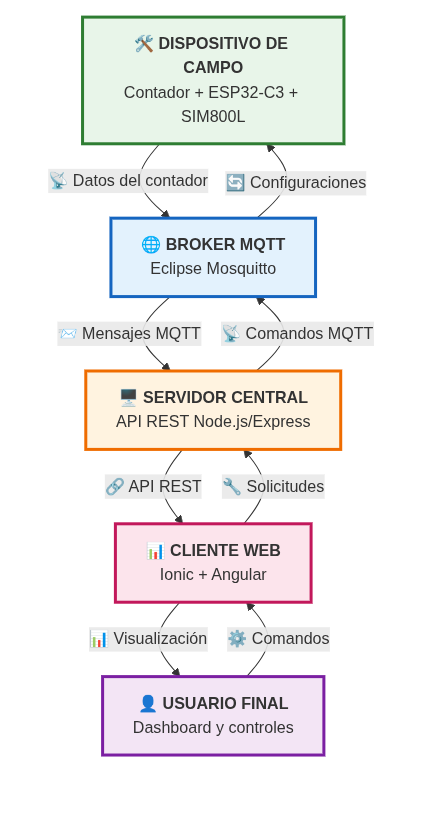
\includegraphics[width=0.4\linewidth]{./Figures/diagArq.png}
  \caption{Diagrama de arquitectura del sistema y el flujo de datos.}
  \label{fig:diag_arquitectura}
\end{figure}


\subsection{Decisiones de diseño clave}

\begin{itemize}

\item Separación broker/aplicación: permite cambiar broker o desplegar uno local sin tocar la lógica de negocio.

\item MQTT para mensajería ligera  porque minimiza overhead en GPRS y facilita pub/sub.

\item API REST en Node.js/Express para exponer endpoints transaccionales y de gestión, centralizando autenticación y control de accesos.
\end{itemize}



\section{Detalle de módulos de hardware}
La implementación del prototipo requiere integrar componentes de hardware que permitan adaptar el sistema de detección de tránsito existente a un modelo de comunicación bidireccional. En esta sección se describen los módulos seleccionados, sus funciones principales, las interfaces involucradas y las consideraciones de integración.


\subsection{ESP32-C3 (unidad de control)}
El ESP32-C3 constituye el núcleo de procesamiento del nodo de campo. Se trata de un microcontrolador de bajo consumo con conectividad, elegido principalmente por su capacidad de cómputo, su soporte de entornos de desarrollo abiertos y la disponibilidad de bibliotecas optimizadas para protocolos de comunicación.

\begin{itemize}

\item Rol en la arquitectura: coordina la recepción de eventos desde el contador a través de RS-232, gestiona el encolamiento FIFO, controla la comunicación con el módem SIM800L mediante comandos AT y actúa como cliente MQTT.

\item Entorno de desarrollo: el firmware se desarrolló sobre ESP-IDF, el framework oficial de Espressif, que permite gestionar tareas concurrentes mediante FreeRTOS y facilita la integración de librerías de red y drivers UART.

\item Ventajas técnicas: bajo costo, consumo reducido, capacidad de ejecutar varias tareas en paralelo y soporte nativo para criptografía y seguridad en comunicaciones.

\item Consideraciones de diseño: se provee una correcta disipación térmica y  estabilidad de la alimentación, especialmente durante la transmisión de datos.

\end{itemize}

\subsection{Módulo GPRS SIM800L}

El módulo SIM800L implementa la conectividad celular GPRS, que permite la transmisión bidireccional de datos entre dispositivos remotos y servidor centralizado.


\begin{itemize}

\item Funciones principales: establecimiento de sesiones TCP/IP sobre GPRS, controlado por el ESP32-C3 mediante comandos AT. Soporta publicación y suscripción MQTT a través de sockets TCP persistentes.

\item Integración con ESP32-C3: la comunicación entre ambos se realiza mediante UART secundaria. El firmware implementa comandos de inicialización, registro en red, apertura de contexto y gestión de reconexiones.

\item Aspectos críticos: el SIM800L presenta picos de consumo que pueden superar los 2 A durante la transmisión, se  dispone de una fuente con suficiente margen y filtros adecuados para evitar reinicios inesperados.

\item Limitaciones: ancho de banda reducido (máximo teórico de 85,6 kbps en GPRS), lo que refuerza la decisión de emplear MQTT por su bajo overhead.

\end{itemize}


\subsection{Contador de tránsito y comunicación RS-232}

El sistema de conteo existente genera tramas con información de los eventos de paso de vehículos acumulados en un intervalo de tiempo (por defecto 1 hora). La comunicación con el ESP32-C3 se establece mediante interfaz RS-232, estándar ampliamente utilizado para transmisión serial de datos.

\begin{itemize}
\item Formato de trama:  el equipo incluye identificador de Dipositivo, timestamp local, valores de clasificación tránsito por carril.

\item Adaptación eléctrica: se utiliza un conversor de niveles (MAX232) para adaptar las señales RS-232 al rango TTL del microcontrolador.

\item Ventaja: la reutilización de la interfaz serial del contador evita modificar el sistema de detección existente, reduciendo costos de integración.


\end{itemize}


En la Figura \ref{fig:foto_dtec} se observa el contador de tránsito. Este dispositivo constituye la base del sistema de detección de eventos y se mantiene sin modificaciones en su lógica interna. 



\begin{figure}[htbp]
  \centering
  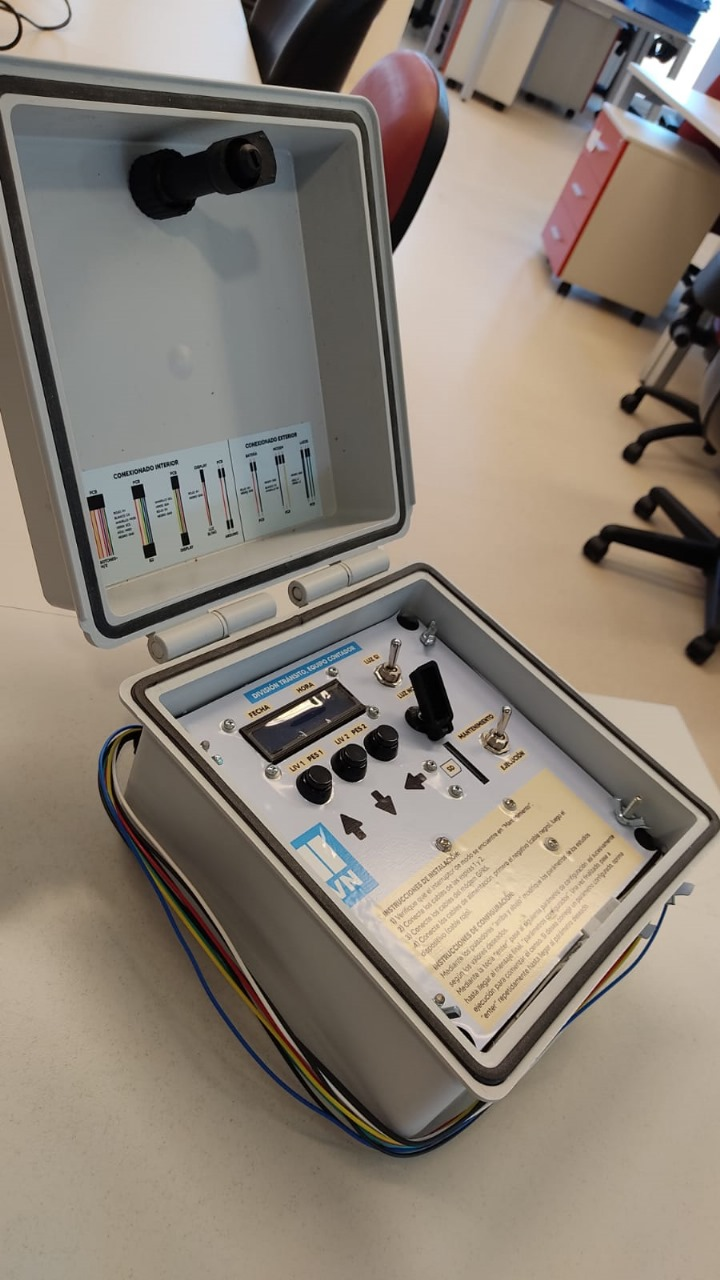
\includegraphics[width=0.5\linewidth]{./Figures/fotoDTEC.jpeg}
  \caption{Fotografia contador de tránsito DTEC \protect\footnotemark.}
  \label{fig:foto_dtec}
\end{figure}

\footnotetext{Imagen tomada de \url{http://transito.vialidad.gob.ar/}}

\subsection{Alimentación y montaje}

El nodo debe operar de manera confiable en condiciones de campo, por lo que la alimentación y el encapsulado son aspectos críticos.

\begin{itemize}
\item Fuente de alimentación: se empleó una fuente principal con batería interna recargable, diseñada para cubrir los picos de consumo del módulo SIM800L. La batería se recarga mediante un panel solar, lo que proporciona autonomía. Para estabilizar la entrega de energía se incorporó un módulo regulador de tensión que garantiza el nivel adecuado de voltaje para el módem. El circuito se complementó con capacitores dimensionados para absorber los picos de tensión del SIM800L durante la transmisión de datos, evitando caídas de voltaje que puedan reiniciar el sistema.


\item Carcasa y Gabinete: tanto el contador como el módulo de comunicación remota (ESP32-C3 y SIM800L) cuentan con su propia carcasa de protección y, adicionalmente, ambos se alojan en un gabinete cerrado con protección ambiental, diseñado para resistir humedad, polvo y vibraciones características de los entornos viales. El uso de un gabinete metálico contribuye también a la disipación térmica y a la reducción de interferencias electromagnéticas, que asegura la confiabilidad del sistema en condiciones de intemperie. 

\end{itemize}

En la Figura \ref{fig:foto_gabinete} se observa el contador de tránsito instalado en campo, junto con su gabinete de protección y la batería interna que asegura autonomía energética. El conjunto se encuentra montado al costado de la ruta, en condiciones reales de operación, lo que permite apreciar el encapsulado diseñado para resistir las exigencias ambientales del entorno vial.


\begin{figure}[htbp]
  \centering
  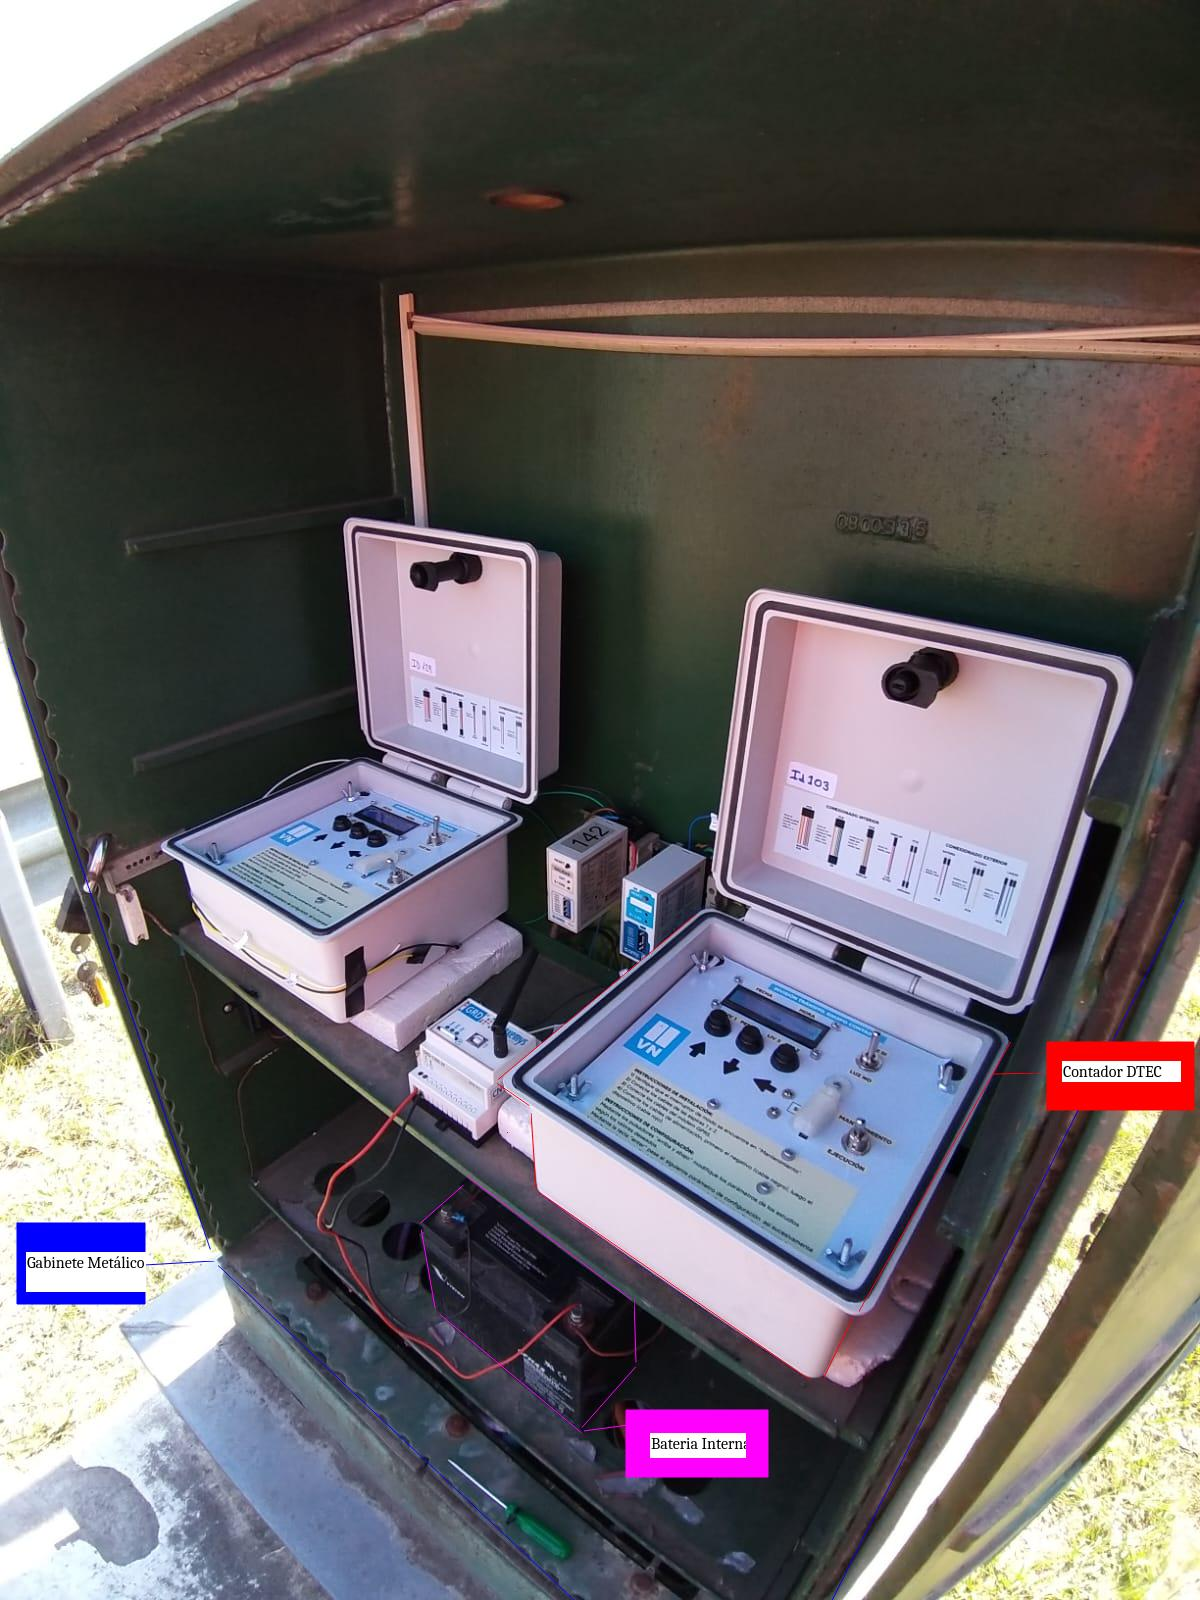
\includegraphics[width=0.85\linewidth]{./Figures/fotoGabinete.jpeg}
  \caption{Fotografia contador de tránsito DTEC instalado en campo \protect\footnotemark.}
  \label{fig:foto_gabinete}
\end{figure}

\footnotetext{Imagen tomada de \url{http://transito.vialidad.gob.ar/}}


\section{Desarrollo del backend}

El backend constituye el núcleo lógico del sistema, encargado de articular la comunicación entre los dispositivos de campo, la base de datos y la interfaz de usuario. Su diseño se basó en principios de modularidad, escalabilidad y seguridad, empleando un conjunto de tecnologías ampliamente utilizadas en entornos de Internet de las Cosas (IoT).


\subsection{Arquitectura y tecnologías}

El servicio fue implementado en Node.js con el framework Express, lo que permitió organizar la aplicación en controladores, rutas y middlewares. Para la interacción con la base de datos relacional se adoptó Sequelize, un ORM que facilita la definición de modelos y garantiza independencia frente a cambios en la capa de persistencia.

La comunicación con los dispositivos se realiza mediante suscripción a tópicos MQTT en el broker Eclipse Mosquitto. 

Cada vez que un dispositivo publica un evento en \texttt{devices/\{id\}/events}, 
el backend lo recibe, valida el payload y lo persiste en MySQL.
 
En el caso de comandos, el backend publica en el tópico correspondiente 
(\texttt{devices/\{id\}/comm}) y actualiza su estado en la base de datos 
conforme recibe las confirmaciones (\texttt{devices/\{id\}/status}).

ara el despliegue y la integración continua se empleó Docker Compose, lo que permite levantar simultáneamente el backend, la base de datos y el broker MQTT en contenedores aislados.

El sistema de registro se implementó con Winston y Morgan, integrados para disponer de trazabilidad tanto de las solicitudes HTTP como de la interacción con MQTT.


\subsection{Funcionalidades principales}

\begin{itemize}
    \item Gestión de dispositivos: alta, baja, modificación y consulta.
    \item Gestión de eventos: almacenamiento de detecciones y consultas filtradas por dispositivo o rango temporal.
    \item Gestión de comandos: emisión de órdenes a un dispositivo, persistencia de la orden con identificador único (cmd\_id) y actualización según respuesta.
    \item Estado de dispositivos: consulta de parámetros como nivel de batería, temperatura o conectividad.
    \item Autenticación y autorización: control de acceso mediante tokens JWT.
\end{itemize}


\subsection{Organización en controladores}

La lógica de negocio del backend se organiza en controladores, cada uno asociado a un recurso del sistema. Esto asegura separación de responsabilidades, facilita el mantenimiento y permite la escalabilidad de la aplicación.

\begin{itemize}
  \item DevicesController: gestiona las operaciones CRUD sobre los dispositivos de campo, además de registrar los eventos recibidos vía MQTT y asociarlos a un dispositivo específico.
  \item EventsController: encapsula la lógica de ingesta de eventos de tránsito, validación de payloads y persistencia en la base de datos.
  \item CommandsController: administra la emisión y seguimiento de comandos remotos, generando un \texttt{cmd\_id} único y actualizando el estado conforme se reciben los \texttt{ack}.
  \item StatusController: centraliza la recepción de estados y telemetría (batería, conectividad), garantizando que la base de datos refleje la situación en tiempo real.
  \item UserController: implementa el ciclo de vida de usuarios y la autenticación mediante JWT, así como la validación de permisos en cada endpoint.
\end{itemize}

\subsection{Mapa de endpoints}
\begin{table}[h]
	\centering
	\caption[Endpoints REST principales]{Endpoints REST principales expuestos por el backend, junto con el controlador que implementa su lógica}
	\begin{tabular}{l l p{7cm}}    
		\toprule
		\textbf{Endpoint} & \textbf{Controlador} & \textbf{Descripción} \\
		\midrule
		GET /devices & DevicesController & Lista todos los dispositivos registrados \\
		GET /devices/\{id\} & DevicesController & Devuelve información de un dispositivo específico \\
		POST /devices & DevicesController & Alta de un nuevo dispositivo \\
		PATCH /devices/\{id\} & DevicesController & Actualización de atributos de un dispositivo \\
		DELETE /devices/\{id\} & DevicesController & Eliminación de un dispositivo \\
		\addlinespace
		GET /events/device/\{id\} & EventsController & Consultar eventos por dispositivo \\
		GET /events/range & EventsController & Consultar eventos por rango temporal \\
		\addlinespace
		POST /commands & CommandsController & Crear un comando remoto y publicarlo en MQTT \\
		GET /commands/\{id\} & CommandsController & Consultar estado de un comando (pendiente, ok, failed, timeout, value) \\
		\addlinespace
		GET /status/\{device\_id\} & StatusController & Consultar estado operativo y telemetría del dispositivo \\
		\addlinespace
		POST /usuario/login & UserController & Autenticación de usuario, devuelve token JWT \\
		POST /usuario & UserController & Alta de usuario \\
		GET /usuario & UserController & Listar usuarios registrados \\
		DELETE /usuario/\{id\} & UserController & Eliminar usuario \\
		\bottomrule
		\hline
	\end{tabular}
	\label{tab:endpoints}
\end{table}


\subsection{Seguridad y extensibilidad}

Además de la autenticación mediante JWT, todos los endpoints aplican validaciones y sanitización de parámetros de entrada y salida. El sistema de logging, implementado con Winston y Morgan, garantiza trazabilidad de las operaciones tanto en la capa HTTP como en la mensajería MQTT. La arquitectura modular basada en controladores permite extender el backend con nuevos recursos o funcionalidades sin afectar la lógica ya implementada.


\section{Desarrollo del frontend}

El frontend del sistema se diseñó como una Single Page Application (SPA) se desarrolla en Ionic con Angular y TypeScript.  
El objetivo es proporcionar una interfaz moderna e intuitiva, accesible desde navegador, que permita al operador autenticarse, supervisar en tiempo real los eventos captados por los contadores de tránsito, consultar históricos almacenados en la base de datos y emitir comandos remotos hacia los nodos de campo.  

\subsection{Arquitectura y tecnologías}

El cliente web se estructura en componentes reutilizables de Ionic, lo que facilita la navegación y asegura un diseño responsivo tanto en entornos de escritorio como móviles.  
La comunicación con el backend se realiza mediante peticiones HTTP a la API REST, y en casos donde se requiere actualización en tiempo real se emplea un canal de notificación basado en WebSocket.

Las tecnologías principales aportan ventajas concretas:
\begin{itemize}
    \item Ionic: conjunto de componentes UI listos para usar que permiten construir pantallas consistentes y adaptables.
    \item Angular: organización de la aplicación en módulos y servicios, favoreciendo la escalabilidad.
    \item TypeScript: tipado estático para mejorar la robustez del código y prevenir errores en tiempo de compilación.
    \item JWT: integración con el backend para autenticar todas las operaciones posteriores al login.
\end{itemize}

\subsection{Funcionalidades principales}

El frontend integra las siguientes funciones clave:
\begin{itemize}
    \item Login de usuario: ingreso con credenciales, validación contra la API y obtención de un token JWT.
    \item Listado de dispositivos: muestra todos los contadores registrados, junto con información de ubicación y estado básico.
    \item Detalle de dispositivo: despliega datos específicos de un contador y últimas tramas recibidas.
    \item Panel de mediciones: permite visualizar los eventos de tránsito procesados, con actualización dinámica cuando el dispositivo transmite nuevas tramas.
    \item Historial de eventos: consulta de registros almacenados en la base de datos, filtrados por dispositivo y rango temporal.
    \item Envío de comandos: panel que habilita la emisión de órdenes remotas al nodo de campo  reset de contador, cambio de parámetros, obtención de parámetros), verificando el acuse de recibo y mostrando el resultado al usuario (\texttt{ok}, \texttt{failed}, \texttt{timeout}, \texttt{value}).
\end{itemize}

\subsection{Integración con el backend}

Todas las operaciones del frontend se apoyan en los endpoints REST definidos en el backend (ver Sección~\ref{tab:endpoints}).  
Cada petición incluye en sus cabeceras el token JWT obtenido en el login, lo que garantiza que sólo usuarios autorizados puedan acceder a datos sensibles o emitir comandos.  
El backend devuelve respuestas en formato JSON, que son interpretadas y representadas en la interfaz en tiempo real, que asegura consistencia entre la vista del operador y el estado real de los dispositivos.

\subsection{Resumen}

El desarrollo del frontend consolidó una interfaz web moderna, accesible y segura que permite a los operadores interactuar con los dispositivos de campo de manera eficiente.  
El sistema ofrece no sólo la visualización de eventos de tránsito en tiempo real y la consulta de históricos, sino también el envío de comandos con acuse de recibo.  
De esta forma, la interfaz completa el ciclo de comunicación bidireccional con los nodos, que se convierte en la herramienta central para la supervisión y el control remoto del prototipo.



\section{Despliegue del sistema}

El despliegue del sistema comprende la puesta en marcha coordinada de los distintos servicios que componen la arquitectura: el broker MQTT, la API REST, la base de datos relacional y la interfaz web.  
El objetivo es trasladar el prototipo desde un entorno de desarrollo hacia un entorno productivo, que asegura escalabilidad, confiabilidad y capacidad de monitoreo post-implantación.  

\subsection{Entorno productivo y configuración}

Para simplificar la orquestación se emplea Docker Compose, lo que permite instanciar todos los servicios en contenedores aislados pero comunicados entre sí.  
Cada componente cumple un rol específico:  

\begin{itemize}
    \item Broker MQTT (Eclipse Mosquitto): configurado como servicio de mensajería central. Se habilitan credenciales de acceso, control de tópicos por dispositivo y soporte de cifrado TLS en despliegues productivos. Su rol es recibir eventos desde los nodos de campo y distribuirlos a los suscriptores autorizados (API REST u otros consumidores).
    
    \item API REST (Node.js/Express): implementada como contenedor independiente, integra lógica de negocio y suscripción al broker MQTT. De esta forma, cada evento recibido es validado, transformado y almacenado en la base de datos. La API expone endpoints para:
    \begin{itemize}
        \item Gestión de dispositivos y usuarios.
        \item Consulta de eventos por rango temporal o por dispositivo.
        \item Emisión y seguimiento de comandos remotos.
        \item Acceso al estado operativo y telemetría de cada nodo.
    \end{itemize}
    Todos los endpoints están protegidos mediante autenticación con tokens JWT.
    
    \item Base de datos relacional (MySQL): instancia dedicada a persistencia de información. Su esquema incluye tablas de dispositivos, eventos, comandos y usuarios. Se definen índices para optimizar consultas históricas y se configuran respaldos automáticos diarios.
    
    \item Interfaz web (Ionic/Angular): desplegada como servicio accesible en navegador. Consume la API REST para mostrar eventos en tiempo real, ejecutar comandos y consultar históricos.
\end{itemize}

\subsection{Monitoreo post-implantación}

Una vez desplegado el sistema, resulta fundamental contar con mecanismos de monitoreo que permitan evaluar su correcto funcionamiento en campo:  

\begin{itemize}
    \item Logs centralizados: tanto el backend como el broker MQTT registran eventos en archivos y consola. Se  integra con Grafana para correlacionar métricas.
    
    \item Alertas y métricas: mediante Grafana es posible recolectar indicadores de CPU, memoria y estado de contenedores. También se pueden graficar métricas de tráfico MQTT (mensajes publicados, latencias, pérdidas).
    
    \item Supervisión de dispositivos: la API REST expone endpoints que informan conectividad y parámetros básicos (nivel de batería, último evento recibido). Estos datos se representan en la interfaz web como panel de salud del sistema.
    
    \item Respaldo y recuperación: la base de datos implementa backups automáticos y permite restauraciones parciales. Esto garantiza que el historial de eventos no se pierda ante fallas de hardware o corrupción de datos.
\end{itemize}

\subsection{Resumen}

El despliegue integra en un único entorno los componentes críticos del sistema: broker MQTT, API REST, base de datos y frontend web.  
La contenedorización mediante Docker Compose simplifica la instalación y favorece la portabilidad hacia distintas plataformas (servidores locales, nubes públicas o entornos híbridos).  
El monitoreo continuo, junto con la gestión de logs y respaldos, asegura que la solución pueda mantenerse operativa de manera confiable en el tiempo, facilitando su escalado y la detección temprana de fallos.




\section{Nodos y Sensores}
\label{sec:nodos-sensores}

\label{sec:nodos-sensores}

En este capítulo se detalla el hardware de los nodos de campo que constituyen la base del sistema de detección de tránsito. Cada nodo combina un microcontrolador \textbf{ESP32-C3} con interfaces de comunicación estándar, lo que permite procesar eventos localmente y establecer un vínculo bidireccional con el servidor central. De esta manera, se logra una solución flexible, escalable y compatible con la infraestructura vial existente.

\subsection{Arquitectura del nodo}
La arquitectura de cada nodo se diseñó con el objetivo de reutilizar los contadores de tránsito actualmente desplegados en rutas nacionales, minimizando modificaciones en el equipamiento existente. Para ello, se emplea una interfaz RS-232 que conecta directamente al contador con el microcontrolador. Dado que el ESP32-C3 opera con niveles de señal TTL, se incorporó un conversor MAX232, encargado de realizar la adaptación de niveles eléctricos y asegurar la robustez de la comunicación.

\begin{itemize}
    \item Contador de tránsito modelo DTEC: dispositivo comercial encargado de detectar el paso de vehículos y generar tramas de datos con la información del evento.
   
En la Figura \ref{fig:foto_dtec} se observa el contador de tránsito. Este dispositivo constituye la base del sistema de detección. 

\begin{figure}[htbp]
  \centering
  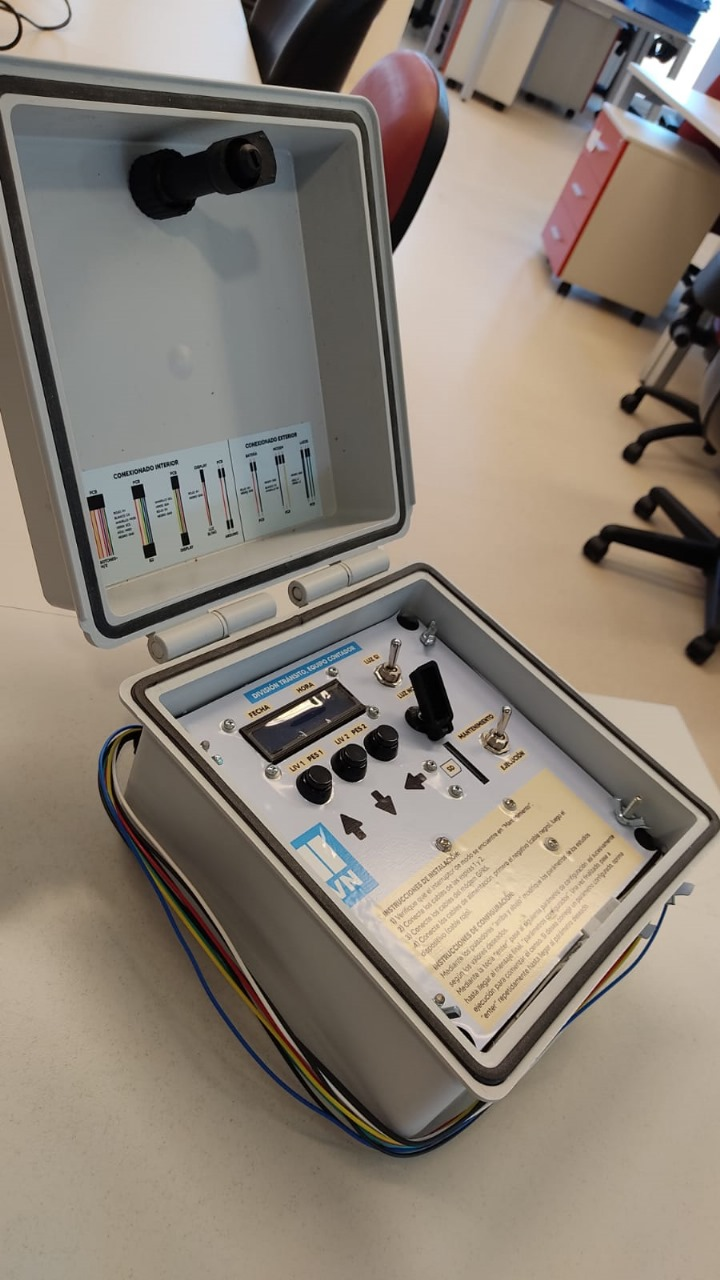
\includegraphics[width=0.5\linewidth]{./Figures/fotoDTEC.jpeg}
  \caption{Contador de tránsito DTEC \protect\footnotemark.}
  \label{fig:foto_dtec}
\end{figure}

\footnotetext{Imagen tomada de \url{http://transito.vialidad.gob.ar/}}   
 
    \item Módulo de adaptación RS-232/TTL (MAX232): circuito de conversión de niveles eléctricos que asegura compatibilidad entre la interfaz serial del contador (RS-232) y el microcontrolador (niveles TTL).
  En la Figura \ref{fig:foto_max232} se observa el Módulo de adaptación RS-232/TTL (MAX232).


  \begin{figure}[htbp]
  \centering
  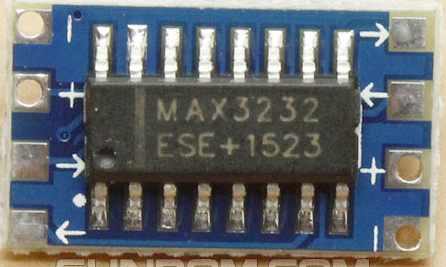
\includegraphics[width=0.4\linewidth]{./Figures/fotoMax232.png}
  \caption{Módulo RS-232/TTL \protect\footnotemark.}
  \label{fig:foto_max232}
\end{figure}

\footnotetext{Imagen tomada de \url{https://www.alldatasheet.com/datasheet-pdf/pdf/73074/MAXIM/MAX232.html}}   
     
    
    \item ESP32-C3: microcontrolador que ejecuta el firmware desarrollado sobre ESP-IDF. Sus funciones incluyen el preprocesamiento de eventos, el encolamiento FIFO, la suscripción a comandos remotos y la gestión integral de la comunicación con el servidor.
   En la Figura \ref{fig:esp32} se muestra el Microntrolador utilizado en campo.

\begin{figure}[htbp]
  \centering
  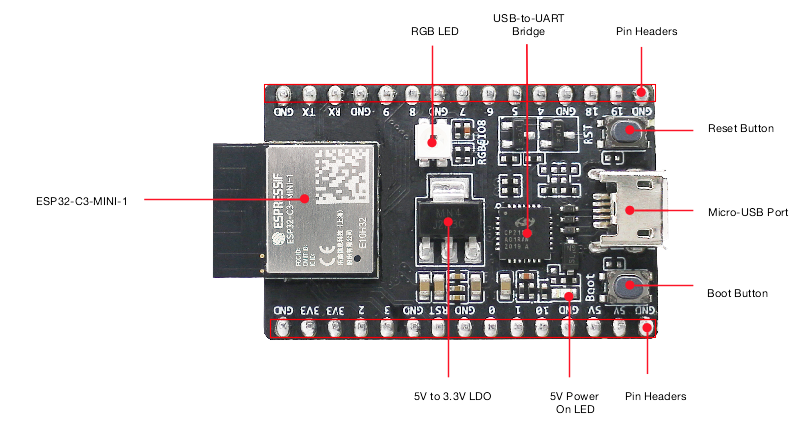
\includegraphics[width=0.85\linewidth]{./Figures/fotoEsp32c3.png}
  \caption{Microcontrolador ESP32-C3 utilizado en los nodos de campo \protect\footnotemark.}
  \label{fig:esp32}
\end{figure}

\footnotetext{Imagen tomada de \url{https://docs.espressif.com/projects/esp-idf/en/v5.0/esp32c3/hw-reference/esp32c3/user-guide-devkitm-1.html}}

    
    \item Módulo de comunicación GPRS (SIM800L): interfaz de conectividad celular que publica eventos en el broker MQTT, recibe comandos desde el servidor y retransmite respuestas o estados del nodo.
    
En la Figura \ref{fig:foto_sim800l} se aprecia el módulo SIM800L que implementa la conectividad celular GPRS.

\begin{figure}[htbp]
  \centering
  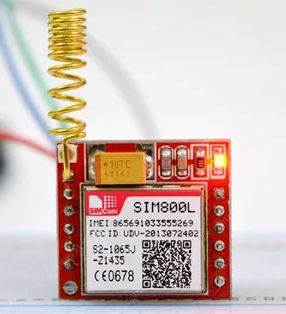
\includegraphics[width=0.4\linewidth]{./Figures/fotoSim800l.png}
  \caption{Módulo SIM800L \protect\footnotemark.}
  \label{fig:foto_sim800l}
\end{figure}

\footnotetext{Imagen tomada de \url{https://www.alldatasheet.com/datasheet-pdf/pdf/1741389/SIMCOM/SIM800L.html}}


\end{itemize}

\subsection{Firmware y comunicación}
El firmware fue desarrollado sobre el framework ESP-IDF, lo que asegura soporte nativo para el hardware del ESP32-C3 y flexibilidad en la gestión de tareas concurrentes. Las principales funciones implementadas son:

\begin{itemize}
    \item Lectura continua de tramas seriales provenientes del contador, con validación y tolerancia a ruido.
    \item Preprocesado de eventos: normalización de campos, inclusión de sello temporal UTC y metadatos de identificación del nodo.
    \item Encolamiento FIFO: los eventos son almacenados temporalmente para garantizar el orden de transmisión incluso ante fallos de conectividad.
    \item Publicación MQTT: envío de eventos hacia el broker en tópicos específicos por dispositivo.
    \item Suscripción a comandos remotos: recepción de órdenes desde el backend, ejecución local y publicación de resultado.
    \item Telemetría: envío periódico de parámetros de estado (nivel de batería, conectividad, temperatura).
\end{itemize}


\subsection{Integración con la infraestructura existente}
Una de las principales ventajas de este diseño es que no requiere modificaciones internas en el contador de tránsito. El nodo recibe los pulsos de detección mediante la interfaz RS-232, que preserva la integridad del equipo original. 

El ESP32-C3 no se limita a reenviar datos, sino que añade valor al sistema al realizar un preprocesado local: filtra tramas, agrupa eventos en función de ventanas de tiempo y asegura la transmisión con políticas de reintento. Asimismo, la conexión con el servidor central mediante MQTT garantiza interoperabilidad con aplicaciones externas y facilita la escalabilidad del sistema.

En este contexto, los nodos de campo cumplen un doble rol: por un lado, son captadores de datos provenientes de los sensores de tránsito y por otro, actúan como puntos de control remoto, capaces de ejecutar comandos enviados desde la plataforma central. Esta dualidad refuerza la flexibilidad del sistema y lo hace adaptable a distintas políticas de gestión vial.



\section{Comunicación del sistema}
\label{sec:comunicacion}

La comunicación constituye un componente esencial en la arquitectura propuesta, ya que habilita el intercambio bidireccional de información entre los nodos de campo y el servidor central. El diseño combina interfaces cableadas locales y protocolos de mensajería ligera sobre redes celulares, que asegura confiabilidad aun en entornos con conectividad limitada.

\subsection{Esquema general}
Cada nodo de campo conecta el contador de tránsito DTEC mediante la interfaz RS-232, que garantiza compatibilidad con el equipamiento existente. El microcontrolador ESP32-C3 recibe las tramas seriales a través de un módulo MAX232, las procesa y las transmite mediante el módulo SIM800L que utiliza conectividad GPRS.  
Sobre esta capa de transporte celular se implementa el protocolo MQTT, lo que permite estructurar la comunicación en un modelo de publicación/suscripción ligero y eficiente.  

De esta manera, el flujo de datos se organiza en dos canales principales:  
\begin{itemize}
    \item Canal de eventos: envío de detecciones desde el nodo hacia el 
    broker MQTT en el tópico \texttt{devices/\{device\_id\}/events}.
    \item Canal de control: recepción de comandos desde el servidor 
    (\texttt{devices/\{device\_id\}/commands}) y envío de confirmaciones o estados 
    (\texttt{devices/\{device\_id\}/status}).
\end{itemize}

\subsection{Flujo de datos}
El proceso de comunicación en operación sigue las siguientes etapas:

\begin{itemize}
    \item Detección local: el contador registra un evento de paso y acumula, en el periodo indicado envía  una trama al ESP32-C3 vía RS-232.
    \item Preprocesamiento: el firmware valida la trama, añade sello temporal y metadatos, y encola el evento en memoria.
    \item Transmisión GPRS/MQTT: cuando existe conectividad, el nodo publica  el evento en el tópico correspondiente.
    \item Ingesta y persistencia: el broker Mosquitto distribuye el mensaje al backend, que valida el contenido y lo almacena en la base de datos MySQL.
    \item Visualización y control: la interfaz web accede a los eventos 
    mediante la API REST y recibe actualizaciones en tiempo real.
    \item Comandos remotos: el operador envía una orden desde la interfaz, el backend la publica en el broker y el nodo la ejecuta, respondiendo con un mensaje de estado o ack.
\end{itemize}

\subsection{Aspectos técnicos}
El diseño incorpora distintas medidas para asegurar la calidad de la comunicación:

\begin{itemize}
    \item MQTT sobre GPRS: se seleccionó este protocolo por su bajo consumo 
    de ancho de banda, adecuado para escenarios con conectividad intermitente.
    \item  RS-232 local: la comunicación serial entre el contador y el 
    microcontrolador garantiza compatibilidad con equipos instalados, con bajo costo 
    y alta robustez en campo.
    \item Autenticación y seguridad: los clientes MQTT se autentican mediante 
    credenciales, y en producción se prevé el uso de cifrado para proteger la 
    integridad de los mensajes.
    \item Persistencia y reintentos: el firmware implementa colas FIFO y 
    retransmisión automática para evitar pérdida de eventos en caso de fallas de red.
    \item Integración con API REST: la capa de aplicación expone endpoints 
    que permiten consultar datos históricos, emitir comandos y gestionar dispositivos, 
    complementando la mensajería en tiempo real.
\end{itemize}

En síntesis, el sistema de comunicación integra tecnologías maduras y abiertas que 
aseguran interoperabilidad, escalabilidad y confiabilidad en condiciones de campo. 
El empleo combinado de RS-232, GPRS y MQTT posibilita modernizar la infraestructura 
existente sin reemplazar los contadores de tránsito, a la vez que habilita la gestión 
remota de dispositivos en escenarios distribuidos.

